\section{Decision Trees [20 pts]}
\begin{enumerate}


\item Consider the dataset in Table \ref{dec_tab} for this problem. Given the four attributes on the left, we want to predict if the student got an A in the course. The following questions involve some computation, so you may want to solve them programmatically. You can find this dataset in \textit{data.txt}

\begin{table}[ht]
\begin{center}
\begin{tabular}{| c | c | c | c || c |} 
\hline
\vtop{\hbox{\strut \textbf{Wakes Up}}\hbox{\strut \textbf{Early}}} & \vtop{\hbox{\strut \textbf{Finished All}}\hbox{\strut \textbf{Homework}}} & \vtop{\hbox{\strut \textbf{Completed}}\hbox{\strut \textbf{Pre-requisites}}} & \textbf{Likes Coffee} & \textbf{A} \\ 
\hline
1 & 1 & 0 & 0 & 0\\ 
\hline
1 & 1 & 1 & 0 & 1\\ 
\hline
0 & 0 & 1 & 0 & 0\\ 
\hline
0 & 1 & 1 & 0 & 1\\ 
\hline
0 & 1 & 1 & 0 & 1\\ 
\hline
0 & 0 & 1 & 1 & 0\\ 
\hline
1 & 0 & 0 & 0 & 0\\ 
\hline
0 & 1 & 0 & 1 & 1\\ 
\hline
0 & 0 & 1 & 0 & 1\\ 
\hline
1 & 0 & 0 & 0 & 0\\ 
\hline
1 & 1 & 1 & 0 & 1\\ 
\hline
0 & 1 & 1 & 1 & 0\\ 
\hline
0 & 0 & 0 & 0 & 0\\ 
\hline
1 & 0 & 0 & 1 & 0\\ 
\hline
\end{tabular}
\end{center}
\caption{decision tree features and labels}
\label{dec_tab}
\end{table}

Create a decision tree of depth 2 using the ID3 algorithm from class. The tree should have the same structure as the diagram in Figure~\ref{fig:tree}. Note that 0 leads to the left branch and 1 leads to the right branch. 
\begin{figure}[ht]
\begin{center}
  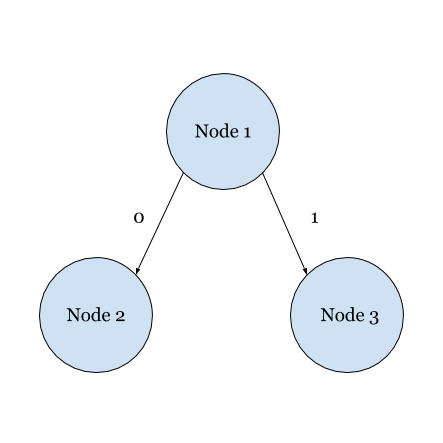
\includegraphics[width=5cm]{images/decisiontree.png}
\end{center}
  \caption{Decision tree structure for question 1}
\label{fig:tree}
\end{figure}
\begin{enumerate}[label=(\roman*)]

\newpage

\item \textbf{[2 pts]} What is the attribute at Node 1? What is the information gain of this attribute? Please round your answer to 4 decimal places.

Attribute to split on: \begin{tcolorbox}[fit,height=1.2cm, width=3.5cm, blank, borderline={1pt}{-2pt}, nobeforeafter, box align = center] \end{tcolorbox}
\hspace{0.5cm} Mutual information: \begin{tcolorbox}[fit,height=1.2cm, width=3.5cm, blank, borderline={1pt}{-2pt}, nobeforeafter, box align = center] \end{tcolorbox} 
 
    
\item \textbf{[2 pts]} What is the attribute at Node 2? What is the information gain of this attribute? Please round your answer to 4 decimal places.

Attribute to split on: \begin{tcolorbox}[fit,height=1.2cm, width=3.5cm, blank, borderline={1pt}{-2pt}, nobeforeafter, box align = center] \end{tcolorbox}
\hspace{0.5cm} Mutual information: \begin{tcolorbox}[fit,height=1.2cm, width=3.5cm, blank, borderline={1pt}{-2pt}, nobeforeafter, box align = center] \end{tcolorbox} 



\item \textbf{[2 pts]} What is the attribute at Node 3? What is the information gain of this attribute? Please round your answer to 4 decimal places. \\
\\
Note: If there is a tie on the attribute with the highest information gain, write any of the attribute that has the highest information gain.

Attribute to split on: \begin{tcolorbox}[fit,height=1.2cm, width=3.5cm, blank, borderline={1pt}{-2pt}, nobeforeafter, box align = center] \end{tcolorbox}
\hspace{0.5cm} Mutual information: \begin{tcolorbox}[fit,height=1.2cm, width=3.5cm, blank, borderline={1pt}{-2pt}, nobeforeafter, box align = center] \end{tcolorbox} 


    
\end{enumerate}

\item \textbf{[4 pts]} Consider learning a decision tree for some binary classification task. Assume that we do not restrict the size of the tree and that the tree can branch multiple times on the same attribute. Under what condition(s) would we be unable to construct a tree that perfectly classifies the dataset?  
\begin{tcolorbox}[fit,height=5cm, width=15cm, blank, borderline={1pt}{-2pt}]
\end{tcolorbox}


\item \textbf{[4 pts]} Assuming that there are no inconsistencies in the data, is the ID3 algorithm guaranteed to output the smallest decision tree that can perfectly classify the training data i.e., achieves zero training error rate? Briefly explain why or why not. \\
\textit{Note:} Inconsistent data is when there are at least two data points $x^{(i)}$ and $x^{(j)}$ with identical feature values, such that $y^{(i)} \neq y^{(j)}$.
\begin{tcolorbox}[fit,height=5cm, width=15cm, blank, borderline={1pt}{-2pt}]
%solution
\end{tcolorbox}


\newpage
\item {\bf [6 Points]} Recall that the information gain of some variable $A$ is the expected reduction in entropy of a target variable $Y$ in some dataset $S$ due to partitioning on $A$. Prove that information gain is always non-negative. To receive full credit, you must show all steps of your work. \textbf{Hint: }You may find the result proved in Recitation 1 regarding the \emph{KL divergence} between two distributions useful for this question.

        \begin{tcolorbox}[fit,height=19cm, width=0.95\textwidth, blank, borderline={1pt}{-2pt}]
  

        \end{tcolorbox}

\end{enumerate}
\newpage

\newpage